%\begin{figure}[!ht]
%\begin{centering}
%
%\subfloat[DFA, state 1.]{ 
%	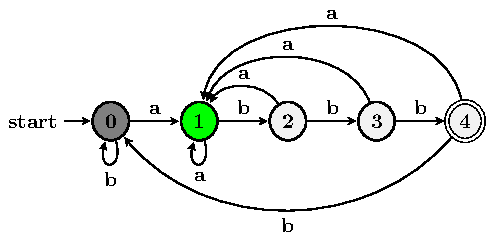
\includegraphics[width=0.1\textwidth]{./figures/forecasting/dfa1.pdf}
%	\label{fig:dfa1}
%}
%
%\subfloat[Waiting-time distribution.]{ 
%	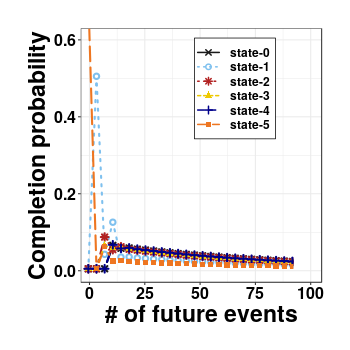
\includegraphics[width=0.1\textwidth,height=.1\textheight]{./figures/wt.png}
%	\label{fig:wt1}
%}
%\caption{Example of how prediction intervals are produced. 
%$\mathcal{P}=a ; d; c$, $\Sigma=\{a,b,c,d\}$, $m=1$, $\theta_{\mathit{fc}}=0.5$.}
%\label{fig:wtdfas}
%\end{centering}
%\end{figure}

\begin{figure}[!ht]
	\begin{centering}
		
		\subfloat[Waiting-time distribution.]{ 
			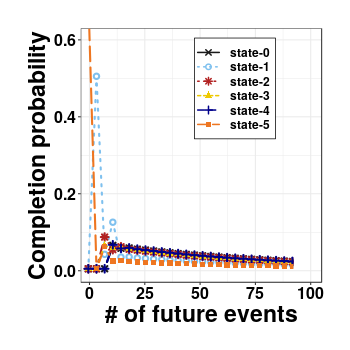
\includegraphics[width=0.25\textwidth]{./figures/wt.png}
			\label{fig:wt1}
		}
		\subfloat[Prediction intervals.]{ 
			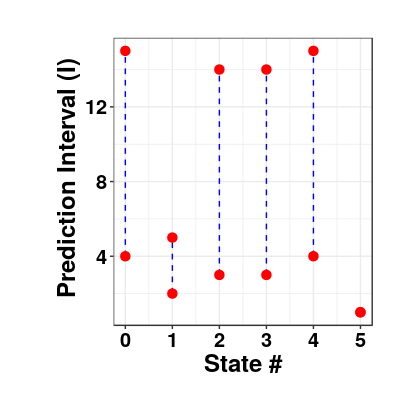
\includegraphics[width=0.25\textwidth]{./figures/predictions.png}
			\label{fig:predictionsIntervals}
		}
		
		\caption{Example of how prediction intervals are produced. 
			$\mathcal{P}=a ; d ; c$, $\Sigma=\{a,b,c,d\}$, $m=1$, $\theta_{\mathit{fc}}=0.5$.}
		\label{fig:wtdfas}
	\end{centering}
\end{figure}